\section{Monte Carlo method}
The goal of a numerical simulation is to estimate the expectation value of some functions $A[\phi]$ of the field variables $[\phi]={\phi_{x\alpha}}$ 
( $\phi_{x\alpha}$ denotes a real fields component with index $\alpha$ at lattice site $x$). \\
\noindent
This is given by path integral as 
$$
  \langle A \rangle = Z^{-1}\int \left[ d\phi \right] e^{-S[\phi]}A[\phi]
$$
$$
  Z=\int \left[ d\phi \right] e^{-S[\phi]}
$$
$S[\phi]$ is the lattice action, which is assumed to be a real function of the field variables. In the case of lattice field systems of interest, the number of 
integration variables in $\left[ d \phi \right] = \displaystyle\prod_{x,\alpha}^{ } d \phi_{x\alpha}$ is very large. \\
\noindent
Apart from trivial system, usually the only possibility is to try a Monte Carlo intgration. \\
\noindent
To perform that computation, let's observe the analogy between classical statistical mechanics and lattice QFT. 
Let's take as example Wilson action of a U(N) lattice gauge field theory with $\phi\rightarrow$U.
$$
    S[U]=\beta\displaystyle\sum_{p}\left( 1 - Tr[U_p] \right)
$$
\noindent
As all the typical lattice action, The Wilson's one contain a summation over the lattice. In order to display only the essential statistical mechanics 
features of the lattice field systems, \cite{QuanField} suggest to write the action as
$$
    S[\phi]=\beta E[\phi]=\Omega\beta\epsilon[\phi]
$$
\noindent
Also Montvay and Müster in \cite{QuanField} to rewrite the statistical mechanic's tools in the following way in order to use the analogy with lattice
field theory for our Monte Carlo integration. \\
\noindent 
In statistical mechanics, $\beta=1/(K_BT)$, but in lattice field theory it's some overall parameter in the action. $E[\phi]$ is the analogous of the energy,
instead $\epsilon[\phi]$ is the analogous of the average energy of each plaquette for gauge fields.\\
\noindent
As consequence of that analogy, is possible define the density of states $D[\epsilon]$ as follow
$$
    D[\epsilon]=e^{-\Omega\epsilon}=\int\left[ d\phi \right]\delta\left( \epsilon - \frac{S(\phi)}{\beta\Omega}\right)
$$
Here $s(\epsilon)$ is a sort of entropy density. Let's so write the partition function $Z=Z_\beta$
$$
    Z_\beta=\int d\epsilon D(\epsilon) e^{-\Omega\beta\epsilon}=\int d\epsilon D(\epsilon) e^{\Omega[s(\epsilon)-\beta\epsilon]}
$$ 
\noindent
This show the probability distribution in $\epsilon$ is
$$
    \rho_\beta=\frac{D(\epsilon)}{Z_\beta}e^{-\Omega\beta\epsilon}=\frac{e^{\Omega[s(\epsilon)-\beta\epsilon]}}{Z_\beta}
$$
\noindent
$s(\epsilon)-\beta\epsilon$ will be the free energy density. Since $\Omega$ is sufficiently large, only a small vicinity of the minimum of the free energy density 
contribute in the path integral. The Monte Carlo simulation have to take this in account by imposing the Boltzmann distribution $exp(-S[\phi])$ to the lattice
configurations.\\
\noindent
So, for a generical observables O, it's possible compute the mean value as follow
 
$$
    <O>=\frac{1}{Z}\displaystyle\sum_{i}O_ie^{-\beta E[\phi_i]}.
$$
\noindent
The sum is over all the microstates $\phi_i$'s , $E[\phi_i]$ the internal energy of the microstate $\phi_i$, $O_i$ are the value 
of the observable on the i-th configurations and Z is the partition function, defined as \cite{CaselleMontecarlo}
$$
      Z=\displaystyle\sum_{i}e^{-\beta E[\phi_i]}.
$$
\noindent
In this way, the computation take into account the Boltmann distribution and all the lattice fields functions are rewritten in terms of statistical tools.
\subsection{Markov chain}
    A Markov chain is defined by the transition probability $p_{ij}$ and by the constraint (probability normalization) \cite{CaselleMontecarlo}
    $$
        \displaystyle\sum_{i}p_{ij}=1.
    $$
    \noindent
    The result does not depend on the j index because, if there isn't transition, when i=j $p_{jj}$=1, when there are transitions the sum of 
    all the possible transitions from i to fixed j have to be =1.
    If we want as stable point of the chain we have to impose the Boltzmann distribution, defined as ... 
    We define $\pi(j)$ as the probability in the Boltzmann distribution. The following condition 
    must be fulfilled:
    $$
        \displaystyle\sum_{j}\pi(j)p_{ji}=\pi(i)
    $$
    Usually this condition is substituted by another one which is more conservative but simpler to handle:
    $$
        \pi(j)p_{ji}=\pi(i)p_{ij}\quad\text{"Detailed}\quad\text{ balance"}
    $$
    This condition implies the previous one and it is equivalent to ask the chain to be reversible. 
    At this point we must find a way to construct the $p_{ij}$ which have $\pi(i)$ as steady state.

    \subsubsection{Markov Chain procedure}
        Starting point: an arbitrary matrix $p^0_{ij}$. The (still unknown) correct matrix $p_{ij}$ will be obtained from $p^0$ as follows:
        $$
            p_{ij}=p^0_{ij}a_{ij}\qquad i\neq j 
        $$
        $$
            p_{ii}=p^0_{ii}+\displaystyle\sum_{i \neq j}p^0_{ij}(1-a_{ij})
        $$
        The idea is to use $p^0$ to propose a transition from i to j which will be accepted with probability $a_{ij}$ and refused with probability 
        $(1 - a_{ij})$. If the transition is refused we have a ”null transition” $i\rightarrow i$.\\
        Thus we end up with the following algorithm: \\
        \begin{enumerate}
            \item Let us start with a configuration i and choose another one j with probability $p^0_{ij}$
            \item Evaluate $E_i$ and $E_j$ (energies of the presente config. and of the proposed one)
            \item If $E_j - E_i \leq 0$ (i.e. if we have a gain in energy) we always accept the new configuration
            \item If $E_j - E_i \geq 0$ (i.e. if we have a loss in energy) we accept the proposed configuration with probability $e^{-\beta(Ej-Ei)}$
        \end{enumerate}

        \subsubsection{Equilibrium}
        Usually, in Monte Carlo simulations, "equilibrium" means that the average probability of finding our system in any particular state $p_n$, is proportional to the Boltzmann weight $e^{-\beta E_n}$. 
        A system at equilibrium spends most of its time in a small subset of states in which its internal energy and other properties take on a narrow range of values. \\
        We might then ask ourself "How can we reach one of these states in the subset"? \\
        In \cite{NewBar} Newman and Barkema, for Ising model simulations, suggest flipping one spin at time, chosen randomly, 
        until the simulation finds the correct sequence of spins flips
        to bring the system into one of the desired states. The algorithm must be designed to simulate equilibrium by imposing the Boltzmann distribution.\\
        Since our theory is pure gauge, the variables are defined over the link. Hence, we flip these variables with a probability $e^{- \beta \Delta E}$, where $\Delta E= E_{iniziale}-E_{finale}$.
        We won't choose the links to split randomly. Thanks to the ergodicity of the system, we can select a fixed sequence for flipping the variables, and this will be equivalent to any random
        sequence.\\
        For semplicity, we take the link in the same order in which they are stored. Once all the links are flipped with a probability $e^{- \beta \Delta E}$, the code saves the 
        internal energy and repeat this process for all links until equilibrium is reached. \\
        Newman and Barkema \cite{NewBar} call the time required to reach the equilibrium $\tau_{eq}$. For 100x100 Ising lattice obtain, they obtained the following graph for magnetization m and
        internal energy u: \\
        \noindent
        \begin{figure}[H]
            \centering
            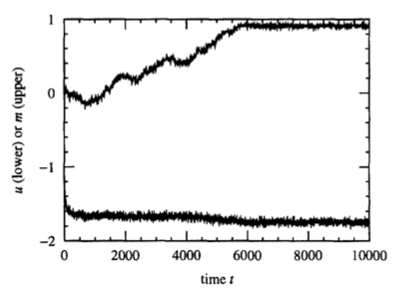
\includegraphics[scale=0.4]{ThermalizationWaBar.png}
            \caption{The magnetization (upper curve) and internal energy (lower curve) 
            per site of a two-dimensional Ising model on a square lattice of 100 x 100 sites with J = 1 
            simulated using the Metropo- lis algorithm}
            \label{fig:NewmanBarkema} 
        \end{figure}

        \noindent
        To lighten the code, we don't save internal energy after each individual split, but only after all the links have been processed. We define an "iteration" as the process of flipping all the links once. \\
        A typical graph obtained for the internal energy density (internal energy/ number of links) by using this procedure is the follows:  
        \noindent
        \begin{figure}[H]
            \centering
            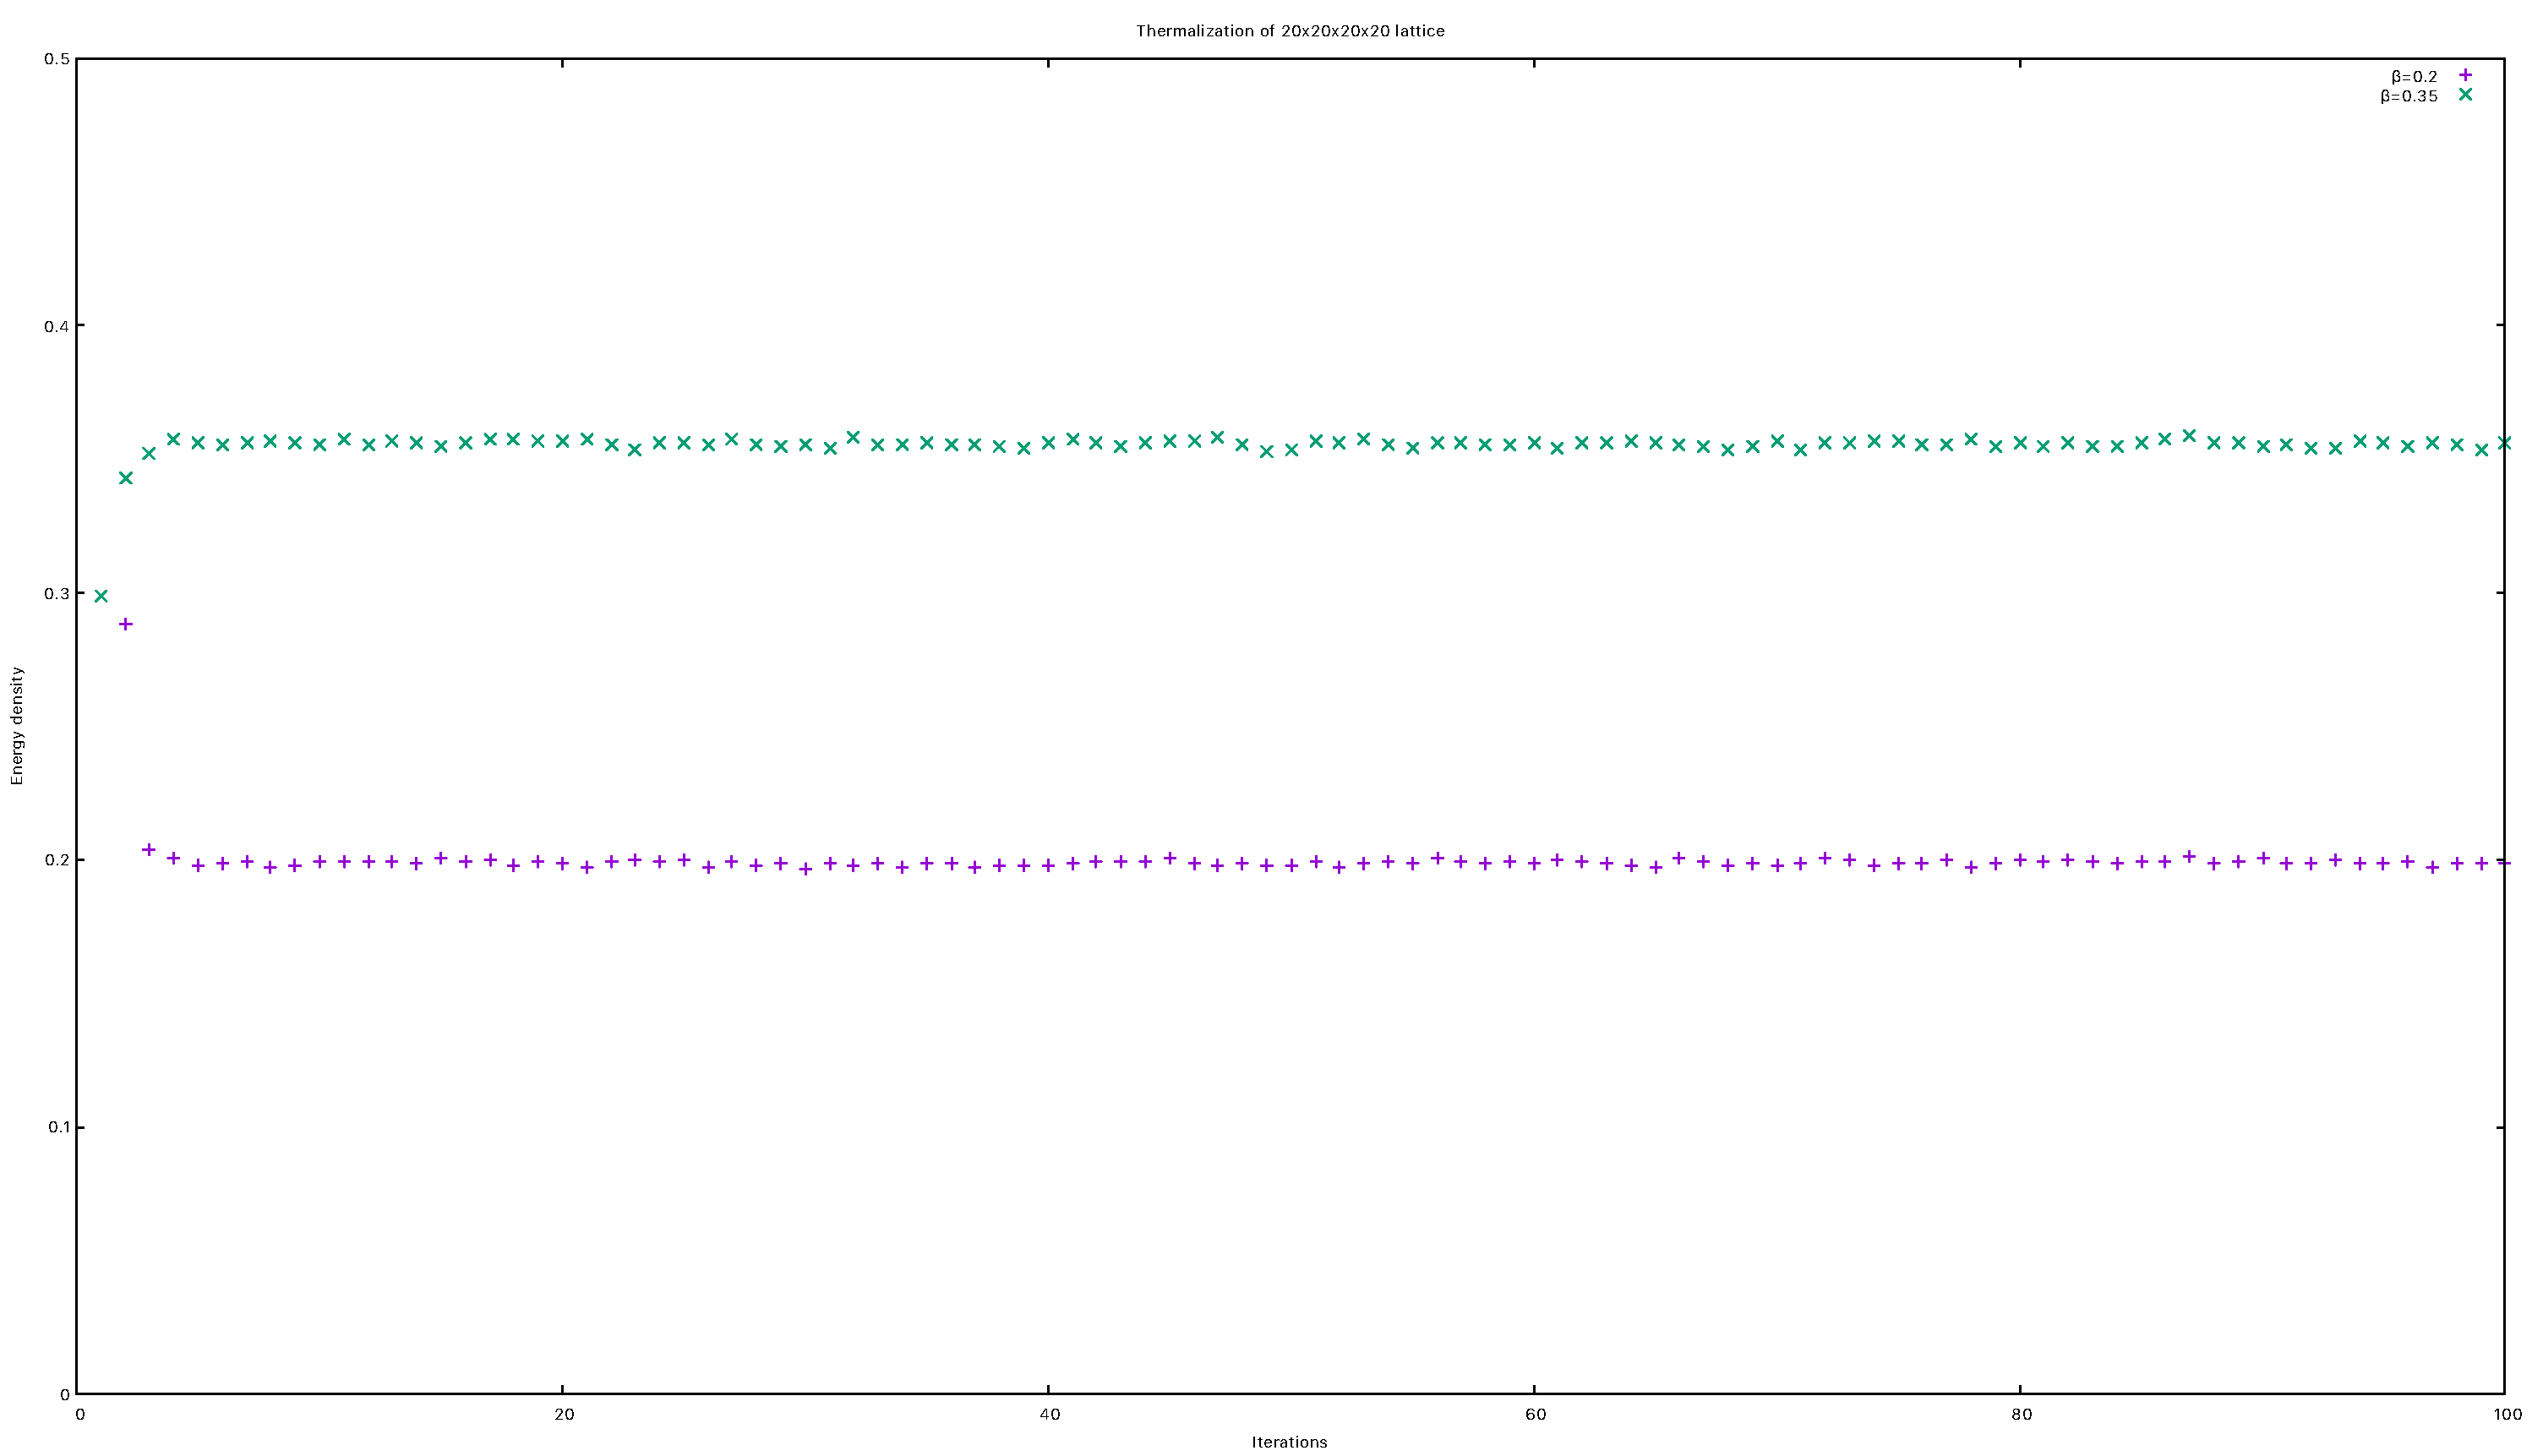
\includegraphics[scale=0.2]{Thermalization3.pdf}
            \caption{Internal energy density at $\beta$=0.2 (purple line) and $\beta$=0.35 (green line) for a 20x20x20x20 lattice gauge.}
            \label{fig:Thermalization} 
        \end{figure}
        \noindent
        We define this sequence of iteration to reach equilibrium "thermalization".\\ 
        Newman and Barkema \cite{NewBar} also suggest to change the initial condition of the system, in order to avoid "false equilibrium". \\
        Because of ergodicity, the subset of equilibrium states depend only to the system, so changing the initial condition change only the time to reach on of these states. \\
        We can watch where the internal energy reach the same approximately constant value in two system where only the initial state is different and obtain
        the $\tau_{eq}$.
        For semplicity, one of the initial condition we will is the " freeze" one, in which all the variables are 1, and a random one. In the follow graph, we can see 
        the results obtained by 2 systems not correctly thermalized and then 2 correctly thermalized.\\

        \noindent
        \begin{figure}[H]
            \centering
            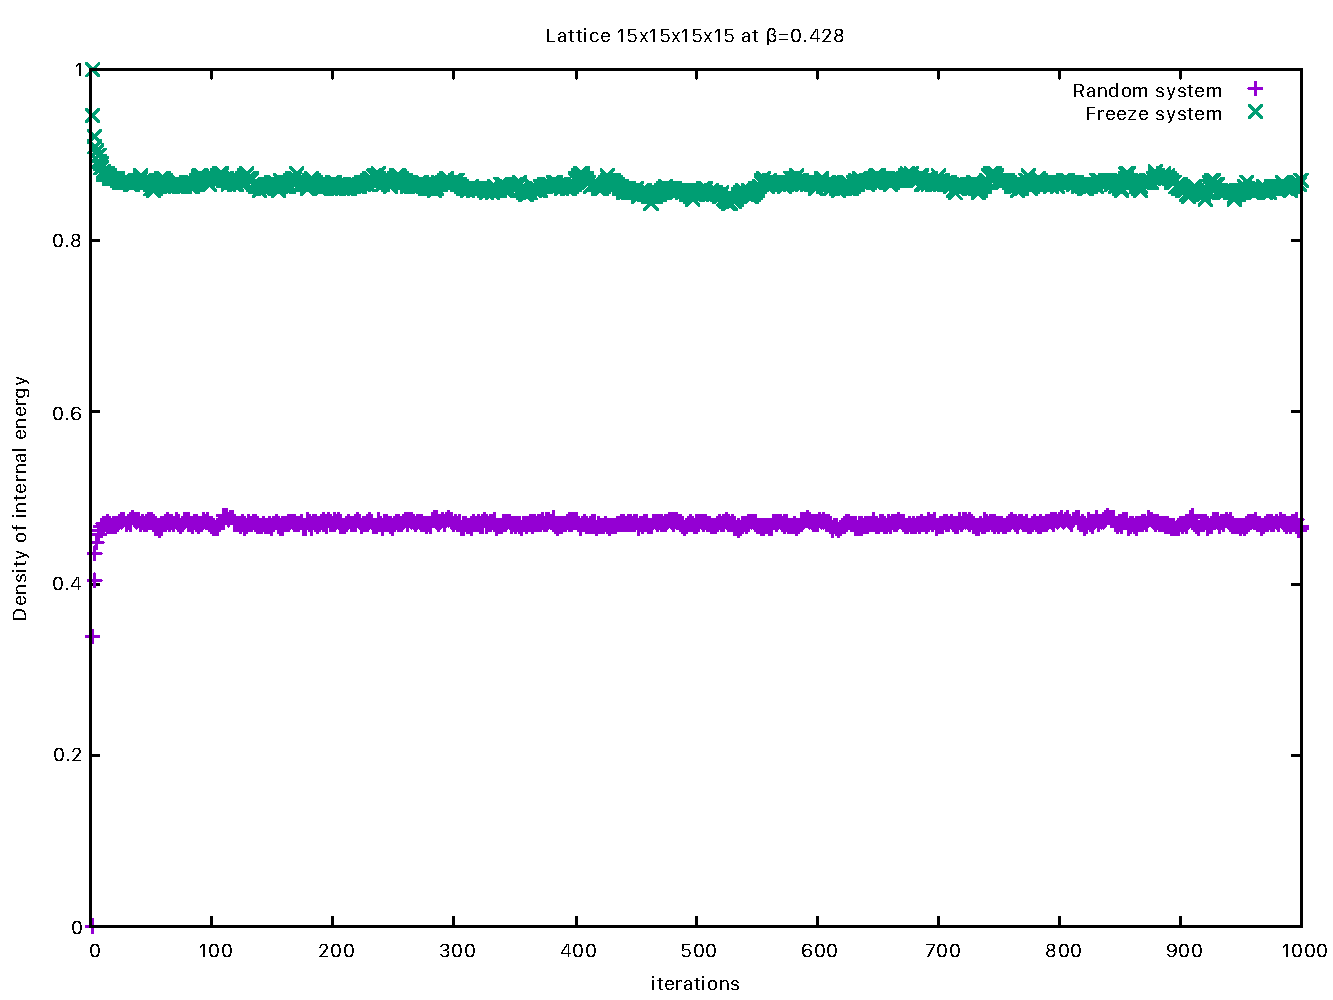
\includegraphics[scale=0.3]{Unthermalization.pdf}
            \caption{As we can observe, the density of internal energy (internal energy/ number of links) for the same ${\beta}$=0.428 is different if we start from 
            a freeze system (green dots) or a random one (purple dots). At least one of them is in a "false equilibrium". }
            \label{fig:Unthermalization} 
            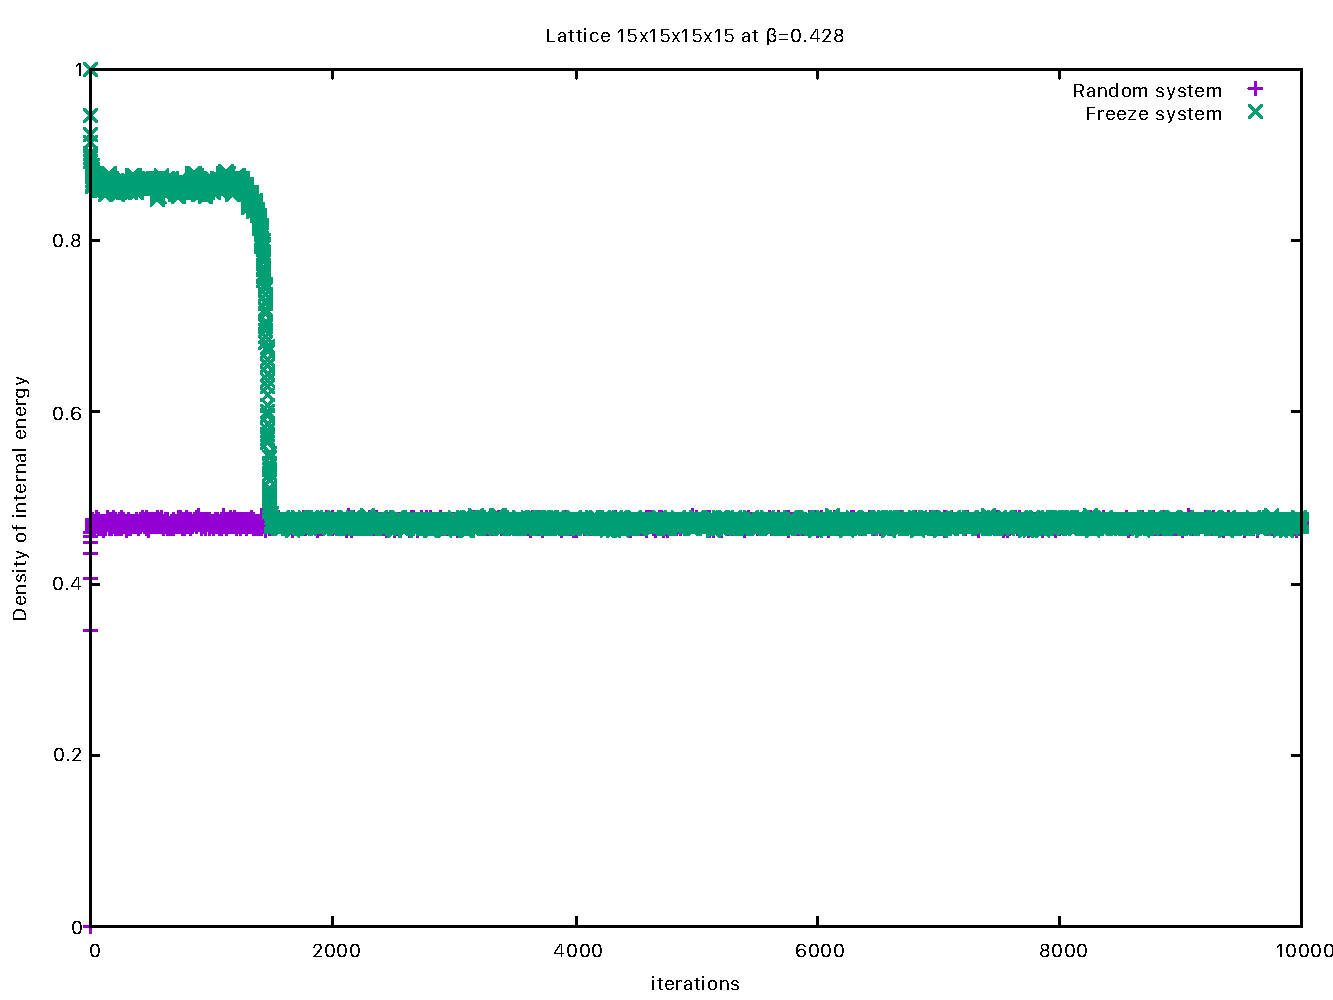
\includegraphics[scale=0.3]{MatchingThermalization.pdf}
            \caption{Increasing the iterations of the systems in \cref{fig:Unthermalization}, we can see that the freezed system was in a false equilibrium.}
            \label{fig:MatchingThermalization}
        \end{figure}


